% 导言区
\documentclass{article} 

% 导入中文宏
\usepackage{ctex}
\usepackage{tikz}

% 构建命令,取别名,使用degree 代替 ^ circ
\newcommand\degree{^\circ}

\title{\heiti 批处理反向传播推导}
\author{\kaishu 乔志健}
\date{\today}
% 正文区
\begin{document}
    \maketitle
	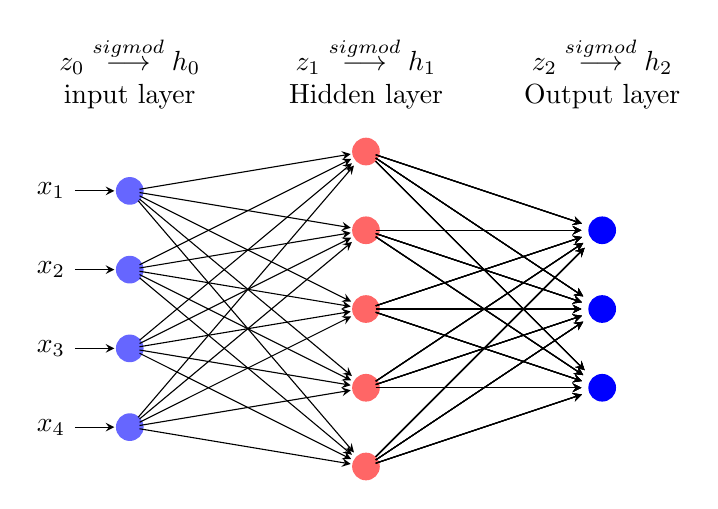
\begin{tikzpicture}[every node/.style={align=center}]
	\foreach \x in{1,2,3,4,5}
	\fill[red!60](0,\x)circle(5pt)node(a\x){};
	\fill[blue!60](-3,1.5)circle(5pt)node(b1){};
	\fill[blue!60](-3,2.5)circle(5pt)node(b2){};
	\fill[blue!60](-3,3.5)circle(5pt)node(b3){};
	\fill[blue!60](-3,4.5)circle(5pt)node(b4){};
	\fill[blue](3,2)circle(5pt)node(c1){};
	\fill[blue](3,3)circle(5pt)node(c2){};
	\fill[blue](3,4)circle(5pt)node(c3){};
	\node(y4)at(-4,4.5){$x_1$};
	\node(y3)at(-4,3.5){$x_2$};
	\node(y2)at(-4,2.5){$x_3$};
	\node(y1)at(-4,1.5){$x_4$};
	\node at(-3,6){$z_0 \stackrel{sigmod}{\longrightarrow} h_0$\\input layer};
	\node at(0,6){$z_1 \stackrel{sigmod}{\longrightarrow} h_1$\\Hidden layer};
	\node at(3,6){$z_2 \stackrel{sigmod}{\longrightarrow} h_2$\\Output layer};
	\foreach \x in{1,2,3,4}
	\draw[-{stealth[sep=2pt]}](y\x)--(b\x);
	\foreach \x in{1,2,3,4}
	{\foreach \y in{1,2,3,4,5}
		{\draw[-{stealth[sep=2pt]}](b\x)--(a\y);
			\foreach \z in{1,2,3}
				{\draw[-{stealth[sep=4pt]}](a\y)--(c\z);}
		}
	}
	\end{tikzpicture}\\
	$$
	z_{0}=\left[                 %左括号
	\begin{array}{cccc}   %该矩阵一共3列,每一列都居中放置
	z_{11} & z_{12} & z_{13} & z_{14}\\  %第一行元素
	\vdots & \vdots & \vdots & \vdots\\  %第一行元素
	z_{n1} & z_{n2} & z_{n3} & z_{n4}\\  %第二行元素
	\end{array}
	\right]_{n\times4}                 %右括号
	$$
	$$h_0=sigmod(z_0)$$
	$$
	z_{1}=\left[                 
	\begin{array}{cccc}  
	h_{11} & h_{12} & h_{13} & h_{14}\\  
	\vdots & \vdots & \vdots & \vdots\\ 
	h_{n1} & h_{n2} & h_{n3} & h_{n4}\\ 
	\end{array}
	\right]_{n\times4} \times \left[                 
	\begin{array}{ccccc}  
	w_{11} & w_{12} & w_{13} & w_{14} & w_{15}\\  
	w_{21} & w_{22} & w_{23} & w_{24} & w_{25}\\  
	w_{31} & w_{32} & w_{33} & w_{34} & w_{35}\\ 
	w_{41} & w_{42} & w_{43} & w_{44} & w_{45}\\ 
	\end{array}
	\right]_{4\times5}+\left[                 
	\begin{array}{ccccc}  
	b^{(1)}_{11} & b^{(1)}_{12} & b^{(1)}_{13} & b^{(1)}_{14} & b^{(1)}_{15}\\  
	\vdots & \vdots & \vdots & \vdots & \vdots\\ 
	b^{(1)}_{n1} & b^{(1)}_{n2} & b^{(1)}_{n3} & b^{(1)}_{n4} & b^{(1)}_{n4}\\ 
	\end{array}
	\right]_{n\times5}
	$$
	$b_{1i}=b_{ni}$
	$$
	h_1=sigmod(z_1)
	$$
	$$
	z_{2}=\left[                 
	\begin{array}{ccccc}  
	h^{(1)}_{11} & h^{(1)}_{12} & h^{(1)}_{13} & h^{(1)}_{14} & h^{(1)}_{15}\\  
	\vdots & \vdots & \vdots & \vdots & \vdots\\ 
	h^{(1)}_{n1} & h^{(1)}_{n2} & h^{(1)}_{n3} & h^{(1)}_{n4} & h^{(1)}_{n4}\\ 
	\end{array}
	\right]_{n\times5} \times \left[                 
	\begin{array}{ccc}  
	w^{(2)}_{11} & w^{(2)}_{12} & w^{(2)}_{13} \\  
	w^{(2)}_{21} & w^{(2)}_{22} & w^{(2)}_{23} \\  
	w^{(2)}_{31} & w^{(2)}_{32} & w^{(2)}_{33} \\ 
	w^{(2)}_{41} & w^{(2)}_{42} & w^{(2)}_{43} \\ 
	w^{(2)}_{41} & w^{(2)}_{42} & w^{(2)}_{43} \\ 
	\end{array}
	\right]_{5\times3}+\left[                 
	\begin{array}{ccccc}  
	b^{(2)}_{11} & b^{(2)}_{12} & b^{(2)}_{13} \\  
	\vdots & \vdots & \vdots \\ 
	b^{(2)}_{n1} & b^{(2)}_{n2} & b^{(2)}_{n3} \\ 
	\end{array}
	\right]_{n\times3}
	$$
	$$
	h^{(2)}=sigmod(z_2)=\left[                 
	\begin{array}{ccc}  
	h^{(2)}_{11} & h^{(2)}_{12} & h^{(2)}_{13} \\  
	\vdots & \vdots & \vdots \\ 
	h^{(2)}_{n1} & h^{(2)}_{n2} & h^{(2)}_{n3} \\ 
	\end{array}
	\right]_{n\times3}
	$$
	$$
	L=loss=0.5\times\sum_{i=1}^n\sum_{j=1}^3(t_{ij}-h^{(2)}_{ij})^2
	$$
	t代表训练集标签
	$$
	\frac{\partial L}{\partial h^{(2)}}=\left[                 
	\begin{array}{ccc}  
	h^{(2)}_{11}-t_{11} & h^{(2)}_{12}-t_{12} & h^{(2)}_{13}-t_{13} \\  
	\vdots & \vdots & \vdots \\ 
	h^{(2)}_{n1}-t_{n1} & h^{(2)}_{n2}-t_{n2} & h^{(2)}_{n3}-t_{n3} \\  
	\end{array}
	\right]_{n\times3}
	$$
	$\frac{\partial L}{\partial z^{(2)}}$的表示
	$$\frac{\partial L}{\partial z^{(2)}}=\frac{\partial L}{\partial h^{(2)}}\frac{\partial h^{(2)}}{\partial z^{(2)}}
	=\left[                 
	\begin{array}{ccc}  
	\frac{\partial L}{\partial z^{(2)}_{11}} & \frac{\partial L}{\partial z^{(2)}_{12}} & \frac{\partial L}{\partial z^{(2)}_{13}} \\  
	\vdots & \vdots & \vdots \\ 
	\frac{\partial L}{\partial z^{(2)}_{n1}} & \frac{\partial L}{\partial z^{(2)}_{n2}} & \frac{\partial L}{\partial z^{(2)}_{n3}}  \\  
	\end{array}
	\right]_{n\times3}
	$$
	$$=\left[                 
	\begin{array}{ccc}  
	h^{(2)}_{11}-t_{11} & h^{(2)}_{12}-t_{12} & h^{(2)}_{13}-t_{13} \\  
	\vdots & \vdots & \vdots \\ 
	h^{(2)}_{n1}-t_{n1} & h^{(2)}_{n2}-t_{n2} & h^{(2)}_{n3}-t_{n3} \\  
	\end{array}
	\right]_{n\times3}\cdot\left[                 
	\begin{array}{ccc}  
	z_{11}^{(2)}(1-z_{11}^{(2)}) & z_{12}^{(2)}(1-z_{12}^{(2)}) & z_{13}^{(2)}(1-z_{13}^{(2)}) \\  
	\vdots & \vdots & \vdots \\ 
	z_{n1}^{(2)}(1-z_{n1}^{(2)}) & z_{n2}^{(2)}(1-z_{n2}^{(2)}) & z_{n3}^{(2)}(1-z_{n3}^{(2)}) \\ 
	\end{array}
	\right]_{n\times3}
	$$
	$z^{(2)}$的线性表示
	$$
	z^{(2)}=\left[                 
	\begin{array}{ccccc}  
	h^{(1)}_{11} & h^{(1)}_{12} & h^{(1)}_{13} & h^{(1)}_{14} & h^{(1)}_{15}\\  
	\vdots & \vdots & \vdots & \vdots & \vdots\\ 
	h^{(1)}_{n1} & h^{(1)}_{n2} & h^{(1)}_{n3} & h^{(1)}_{n4} & h^{(1)}_{n4}\\ 
	\end{array}
	\right]_{n\times5} \times \left[                 
	\begin{array}{ccc}  
	w^{(2)}_{11} & w^{(2)}_{12} & w^{(2)}_{13} \\  
	w^{(2)}_{21} & w^{(2)}_{22} & w^{(2)}_{23} \\  
	w^{(2)}_{31} & w^{(2)}_{32} & w^{(2)}_{33} \\ 
	w^{(2)}_{41} & w^{(2)}_{42} & w^{(2)}_{43} \\ 
	w^{(2)}_{41} & w^{(2)}_{42} & w^{(2)}_{43} \\ 
	\end{array}
	\right]_{5\times3}+\left[                 
	\begin{array}{ccccc}  
	b^{(2)}_{11} & b^{(2)}_{12} & b^{(2)}_{13} \\  
	\vdots & \vdots & \vdots \\ 
	b^{(2)}_{n1} & b^{(2)}_{n2} & b^{(2)}_{n3} \\ 
	\end{array}
	\right]_{n\times3}
	$$
	$$
	=\left[                 
	\begin{array}{ccc}  
	z^{(2)}_{11} & z^{(2)}_{12} & z^{(2)}_{13} \\  
	\vdots & \vdots & \vdots \\ 
	z^{(2)}_{n1} & z^{(2)}_{n2} & z^{(2)}_{n3} \\ 
	\end{array}
	\right]_{n\times3}
	$$
	$$\frac{\partial L}{\partial w^{(2)}}=\left[                 
	\begin{array}{ccc}  
	\frac{\partial L}{\partial w^{(2)}_{11}} & \frac{\partial L}{\partial w^{(2)}_{12}} & \frac{\partial L}{\partial w^{(2)}_{13}} \\  
	\frac{\partial L}{\partial w^{(2)}_{21}} & \frac{\partial L}{\partial w^{(2)}_{22}} & \frac{\partial L}{\partial w^{(2)}_{23}} \\  
	\frac{\partial L}{\partial w^{(2)}_{31}} & \frac{\partial L}{\partial w^{(2)}_{32}} & \frac{\partial L}{\partial w^{(2)}_{33}} \\ 
	\frac{\partial L}{\partial w^{(2)}_{41}} & \frac{\partial L}{\partial w^{(2)}_{42}} & \frac{\partial L}{\partial w^{(2)}_{43}} \\ 
	\frac{\partial L}{\partial w^{(2)}_{41}} & \frac{\partial L}{\partial w^{(2)}_{42}} & \frac{\partial L}{\partial w^{(2)}_{43}} \\ 
	\end{array}
	\right]_{5\times3}$$
	$$
	\frac{\partial L}{\partial w^{(2)}_{11}}=\sum_{i=1}^n\frac{\partial L}{\partial z^{(2)}_{i1}}h^{(1)}_{i1}
	$$
	以此类推
	$$\frac{\partial L}{\partial w^{(2)}}=
	\left[ \begin{array}{ccc}  
	h^{(1)}_{11} & \cdots & h^{(1)}_{n1} \\
	h^{(1)}_{12} & \cdots & h^{(1)}_{n2} \\
	h^{(1)}_{13} & \cdots & h^{(1)}_{n3} \\
	h^{(1)}_{14} & \cdots & h^{(1)}_{n4} \\
	h^{(1)}_{15} & \cdots & h^{(1)}_{n5} \\
	\end{array}	\right]_{5\times n}\times \left[                 
	\begin{array}{ccc}  
	\frac{\partial L}{\partial z^{(2)}_{11}} & \frac{\partial L}{\partial z^{(2)}_{12}} & \frac{\partial L}{\partial z^{(2)}_{13}} \\  
	\vdots & \vdots & \vdots \\ 
	\frac{\partial L}{\partial z^{(2)}_{n1}} & \frac{\partial L}{\partial z^{(2)}_{n2}} & \frac{\partial L}{\partial z^{(2)}_{n3}}  \\  
	\end{array}
	\right]_{n\times3}=((h^{(1)})^T \times \frac{\partial L}{\partial z^{(2)}} 
	$$
	L对b的求导
	$$
	\frac{\partial L}{\partial b^{(2)}}=\left[                 
	\begin{array}{c}
	\frac{\partial L}{\partial b^{(2)}_{1}} \\  
	\frac{\partial L}{\partial b^{(2)}_{2}} \\  
	\frac{\partial L}{\partial b^{(2)}_{3}} \\  
	\end{array}
	\right]_{3\times1}=\left[                 
	\begin{array}{c}
	\sum_{i=1}^n\frac{\partial L}{\partial z^{(2)}_{i1}} \\  
	\sum_{i=1}^n\frac{\partial L}{\partial z^{(2)}_{i2}} \\  
	\sum_{i=1}^n\frac{\partial L}{\partial z^{(2)}_{i3}} \\  
	\end{array}
	\right]_{3\times1}
	$$
	L对$h^{}(1)$的导数,可由L对$w^{}(2)$的导数联想得到(观察$z^{(2)}$的线性表示)
	$$\frac{\partial L}{\partial h^{(1)}}=\left[                 
	\begin{array}{ccc}  
	\frac{\partial L}{\partial z^{(2)}_{11}} & \frac{\partial L}{\partial z^{(2)}_{12}} & \frac{\partial L}{\partial z^{(2)}_{13}} \\  
	\vdots & \vdots & \vdots \\ 
	\frac{\partial L}{\partial z^{(2)}_{n1}} & \frac{\partial L}{\partial z^{(2)}_{n2}} & \frac{\partial L}{\partial z^{(2)}_{n3}}  \\  
	\end{array}
	\right]_{n\times3}\times \left[                 
	\begin{array}{ccccc}  
	w^{(2)}_{11} & w^{(2)}_{21} & w^{(2)}_{31} &w^{(2)}_{41} &w^{(2)}_{51} \\  
	w^{(2)}_{12} & w^{(2)}_{22} & w^{(2)}_{32} &w^{(2)}_{42} &w^{(2)}_{52} \\  
	w^{(2)}_{13} & w^{(2)}_{23} & w^{(2)}_{33} &w^{(2)}_{43} &w^{(2)}_{53} \\  
	\end{array}
	\right]_{3\times5}=\frac{\partial L}{\partial z^{(2)}} \times (w^{(2)})^T
	$$
	
\end{document}